\documentclass[english,ignorenonframetext]{beamer}

% Compile with XeLaTeX:
\usepackage{fontspec}
\setmainfont{Liberation Serif}

\usetheme{Warsaw}
\setbeamercovered{transparent}
\setbeamertemplate{navigation symbols}{}
\usepackage{multirow}
\usepackage{booktabs}
\newcommand{\autor}{Jakson Alves de Aquino}
\newcommand{\titulo}{Communication between Vim and R}

\title{\titulo}
\author{\autor}
\date{\today}

\usepackage{tikz}
\date{\today}
\begin{document}

\begin{frame}[plain]
  \titlepage
\end{frame}

\begin{frame}
\frametitle{The R package \texttt{vimcom}}
\begin{center}
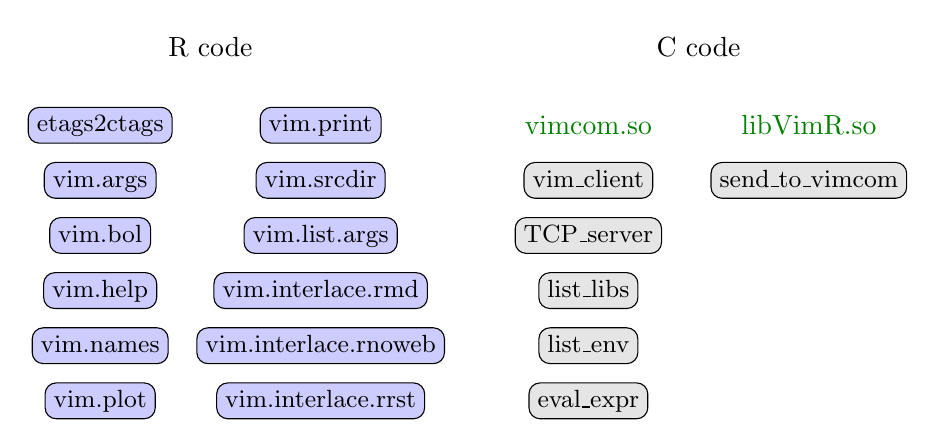
\begin{tikzpicture}[node distance=5mm,
    bola/.style={
        rectangle,minimum size=4mm,rounded corners,
        draw, fill=white!80!blue,
        text height=1.5ex,text depth=.25ex
    }]
    \normalsize
    \node at (3.4, 8) {R code};
    \node at (9.6, 8) {C code};
    \node at (8.2, 7) {\textcolor{black!50!green}{vimcom.so}};
    \node at (11, 7) {\textcolor{black!50!green}{libVimR.so}};

    \small
    \node [bola] at (2, 7.0) {etags2ctags}; \node [bola] at (4.8, 7.0) {vim.print};
    \node [bola] at (2, 6.3) {vim.args};    \node [bola] at (4.8, 6.3) {vim.srcdir};
    \node [bola] at (2, 5.6) {vim.bol};     \node [bola] at (4.8, 5.6) {vim.list.args};
    \node [bola] at (2, 4.9) {vim.help};    \node [bola] at (4.8, 4.9) {vim.interlace.rmd};
    \node [bola] at (2, 4.2) {vim.names};   \node [bola] at (4.8, 4.2) {vim.interlace.rnoweb};
    \node [bola] at (2, 3.5) {vim.plot};    \node [bola] at (4.8, 3.5) {vim.interlace.rrst};

    \node [bola, fill=white!90!black] at (8.2, 6.3) {vim\_client};
    \node [bola, fill=white!90!black] at (8.2, 5.6) {TCP\_server};
    \node [bola, fill=white!90!black] at (8.2, 4.9) {list\_libs};
    \node [bola, fill=white!90!black] at (8.2, 4.2) {list\_env};
    \node [bola, fill=white!90!black] at (8.2, 3.5) {eval\_expr};

    \node [bola, fill=white!90!black] at (11, 6.3) {send\_to\_vimcom};
    \normalsize
\end{tikzpicture}
\end{center}
\end{frame}


\begin{frame}
\frametitle{Vim--R communication paths}
\begin{center}
    \begin{tikzpicture}
        \normalsize
        \draw [thick, fill=white!90!green, rounded corners] (7, 1.5) rectangle (10, 6.5);
        \draw [thick, fill=white!90!green, rounded corners] (0, 1.5) rectangle (3, 6.5);
        \only<1>{
            \node at (1.5, 4) {Vim Editor};
            \node at (8.5, 4) {R};
        }
        \only<2>{
            \node at (1.5, 4) {MacVim Editor};
            \node at (8.5, 4) {R.app};
        }
        \only<3>{
            \node at (1.5, 4) {GVim Editor};
            \node at (8.5, 4) {Rgui};
        }
        \small
        \draw (0, 3) -- (3, 3);
        \draw (0, 5) -- (3, 5);
        \footnotesize
        \only<1>{
            \node at (1.5, 6.1) {\texttt{\textcolor{black!50!green}{X11}}};
            \node at (8.5, 6.1) {\texttt{\textcolor{black!50!green}{vimcom.so}}};
            \node at (8.5, 2.6) {\texttt{\textcolor{black!50!green}{vimcom.so}}};
            \node at (1.5, 2.6) {\texttt{\textcolor{black!50!green}{libVimR.so}}};
            \node at (5, 4.3) {\emph{via tmux}};
        }
        \only<2>{
            \node at (1.5, 6.1) {\texttt{\textcolor{black!50!green}{Cocoa}}};
            \node at (8.5, 6.1) {\texttt{\textcolor{black!50!green}{system()}}};
            \node at (8.5, 2.6) {\texttt{\textcolor{black!50!green}{vimcom.so}}};
            \node at (1.5, 2.6) {\texttt{\textcolor{black!50!green}{libVimR.so}}};
            \node at (5, 4.3) {\emph{via osascript}};
        }
        \only<3>{
            \node at (1.5, 6.1) {\texttt{\textcolor{black!50!green}{Windows}}};
            \node at (8.5, 6.1) {\texttt{\textcolor{black!50!green}{vimcom.dll}}};
            \node at (8.5, 2.6) {\texttt{\textcolor{black!50!green}{vimcom.dll}}};
            \node at (1.5, 2.6) {\texttt{\textcolor{black!50!green}{libVimR.dll}}};
            \node at (5, 4.3) {\emph{via clipboard}};
        }

        \small
        \only<1>{ \node at (1.5, 5.6) {Vim's server}; }
        \only<2>{ \node at (1.5, 5.6) {MacVim's server}; }
        \only<3>{ \node at (1.5, 5.6) {GVim's server}; }
        \node at (1.5, 2.1) {TCP client};

        \draw (7, 3) -- (10, 3);
        \draw (7, 5) -- (10, 5);
        \only<1>{ \node at (8.5, 5.6) {X11 client}; }
        \only<2>{ \node at (8.5, 5.6) {Vim application}; }
        \only<3>{ \node at (8.5, 5.6) {Windows client}; }
        \node at (8.5, 2.1) {TCP server};

        \footnotesize
        \draw [->, thick] (3.1, 4.1) -- (6.9, 4.1);
        \draw [->, thick, blue] (-0.1, 3.8) .. controls (-0.8, 3.8) and (-0.8, 2.25) .. (-0.1, 2.25);
        \draw [->, thick, red] (-0.1, 5.75) .. controls (-0.8, 5.75) and (-0.8, 4.2) .. (-0.1, 4.2);
        \draw [->, thick, red] (8.5, 6.6) .. controls (8.5, 7.5) and (1.5, 7.5) .. (1.5, 6.6);
        \draw [->, thick, blue] (1.5, 1.4) .. controls (1.5, 0.5) and (8.5, 0.5) .. (8.5, 1.4);

        \node [shape=circle, text width=1.5cm, align=center, blue] (tmpf) at (4.5, 2.25) {Temporary files};
        \draw [->, thick, blue] (6.9, 2.25) -- (tmpf) node[above, midway] {\emph{write}};
        \draw [->, thick, blue] (tmpf) -- (3.1, 3.9) node[above, sloped, midway] {\emph{read}};
        \normalsize
    \end{tikzpicture}
\end{center}
\end{frame}

\begin{frame}
\frametitle{Vim--R communication paths}
  \frametitle{}
  \begin{columns}
    \column{.50\textwidth}
    \textbf{Black path}
    \begin{itemize}
      \item The code that you see being pasted into R Console
    \end{itemize}
    \vspace{0.2cm}
    \textcolor{red}{\textbf{Red path}}
    \begin{itemize}
      \item Update synxtax highlight
      \item Update Object Browser
      \item \texttt{help()} typed in the R Console
      \item Open PDF (Rnoweb)
    \end{itemize}
    \column{.50\textwidth}
    \textcolor{blue}{\textbf{Blue path}}
    \begin{itemize}
      \item Omnicompletion
      \item Completion of function arguments
      \item \texttt{:Rhelp} or \texttt{<LocalLeader>rh}
      \item \texttt{:Rinsert}
      \item \texttt{:Rformat}
    \end{itemize}
  \end{columns}
\end{frame}

\end{document}
